\documentclass[11pt,a4paper]{article}
\usepackage[dvipsnames]{xcolor}
\usepackage{amsmath,tabularx,geometry,graphicx,multirow,tikz,listings,xfrac}

\usetikzlibrary{positioning}
\newdimen\nodeDist
\nodeDist=35mm
\geometry{a4paper, left=20mm, top=20mm}
\graphicspath{{../imgs/}}
\newcommand\sbullet[1][.5]{\mathbin{\vcenter{\hbox{\scalebox{#1}{$\bullet$}}}}}
\newcommand{\circo}{~\raisebox{1pt}{\tikz \draw[line width=0.5pt] circle(1.1pt);}~}
\newenvironment{psmallmatrix}
  {\left(\begin{smallmatrix}}
  {\end{smallmatrix}\right)}

\title{Aprendizagem 2021/22 Homework IV - Group 66}
\author{João Cardoso, 99251. José João Ferreira, 99259}

\begin{document}

\color{darkgray}
\hspace{-8.25mm}
\renewcommand\tabularxcolumn[1]{m{#1}}
\begin{tabularx}{1.09\textwidth} {>{\raggedright\arraybackslash}X >{\centering\arraybackslash}X >{\raggedleft\arraybackslash}X}
  
\includegraphics[scale=0.2]{tecnico.pdf}                           &
  \textbf{Aprendizagem 2022/23} \par \textbf{Homework IV - Group 66} &
  João Cardoso, 99251 \par José João Ferreira, 99259
\end{tabularx}
\renewcommand\tabularxcolumn[1]{p{#1}}
\color{black}

\begin{center}
  \textbf{I. Pen-and-paper}
\end{center}

% PROBLEM 1
\begin{flushleft}
  \textbf{1)}
  \small
  \begin{tabularx}{1.09\textwidth}{X X}
    {$\sbullet$ training data: \par
      \begin{tabular}{c|cc}
              & $y_1$ & $y_2$ \\ \hline
        $x_1$ & 1     & 2     \\ \hline
        $x_2$ & -1    & 1     \\ \hline
        $x_3$ & 1     & 0
      \end{tabular}
      \begin{flalign*}
         & \sbullet \text{initialization centroids:}                                                                                              &  & \\
         & \mu_1 = \begin{pmatrix} 2 \\ 2 \end{pmatrix} \quad\quad \Sigma_1 = \begin{pmatrix} 2 & 1 \\ 1 & 2 \end{pmatrix} \quad\quad \pi_1 = 0.5 &  & \\
         & \mu_2 = \begin{pmatrix} 0 \\ 0 \end{pmatrix} \quad\quad \Sigma_2 = \begin{pmatrix} 2 & 0 \\ 0 & 2 \end{pmatrix} \quad\quad \pi_2 = 0.5 &  & \\
      \end{flalign*}}
     &
    {\vspace{-11mm} \begin{flalign*}
                           & \sbullet \text{priors:}    &  & \\
                           & p \, (c = 1) = \pi_1 = 0.5 &  & \\
                           & p \, (c = 2) = \pi_2 = 0.5 &  & \\
                        \end{flalign*}
        \vspace{-12mm} \begin{flalign*}
                          & \sbullet \text{likelihoods:}                                                                                                                                               &  & \\
                          & p \, (x \: | \: c = 1) = \mathcal{N}(x \: | \: \mu_1 = \begin{psmallmatrix} 2 \\ 2 \end{psmallmatrix}, \Sigma_1  = \begin{psmallmatrix} 2 & 1 \\ 1 & 2 \end{psmallmatrix}) &  & \\
                          & p \, (x \: | \: c = 2) = \mathcal{N}(x \: | \: \mu_2 = \begin{psmallmatrix} 0 \\ 0 \end{psmallmatrix}, \Sigma_2  = \begin{psmallmatrix} 2 & 0 \\ 0 & 2 \end{psmallmatrix}) &  & \\
                       \end{flalign*}
        \vspace{-12mm} \begin{flalign*}
                          & \sbullet \text{determinant and inverse of a matrix:}                                                                                                                                           &  & \\
                          & det\begin{pmatrix} a & b \\ c & d \end{pmatrix} = ad - bc \quad\quad\quad {\begin{pmatrix} a & b \\ c & d \end{pmatrix}}^{-1} \! = \frac{1}{det}\begin{pmatrix} d & -b \\ -c & a \end{pmatrix} &  & \\
                       \end{flalign*}}
  \end{tabularx}
  \vspace{-15mm} \begin{flalign*}
     & \sbullet \text{multivariate gaussian:}                                                                                                                                                                  &  & \\
     & \mathcal{N}(x \: | \: \mu, \Sigma) = \frac{1}{(2\pi)^{\sfrac{d}{2}} \cdot \sqrt{det(\Sigma)}} e^{-\frac{1}{2}(x-\mu)^T \Sigma^{-1}(x-\mu)}, \quad \text{where \textit{d} is the dimension of the space} &  & \\
  \end{flalign*}
  \vspace{-9mm} \begin{flalign*}
     & \sbullet \text{Bayes rule:}                                                                                                                                                                          &  & \\
     & p \, (cluster = k \: | \: x) = \frac{p \, (x \: | \: c = k) \cdot p \, (c = k)}{p \, (x)}, \quad \text{where} \ p \, (x) = \sum_{k=1}^\mathcal{K} \pi_k \cdot \mathcal{N}(x \: | \: \mu_k, \Sigma_k) &  & \\
  \end{flalign*}
  \normalsize
  \par $\sbullet$ \underline{E-Step: assign each point to the cluster that yields higher posterior} \par
  \small
  \vspace{-3mm} \begin{flalign*}
     & det(\Sigma_1) = det\begin{pmatrix} 2 & 1 \\ 1 & 2 \end{pmatrix} = 2 \times 2 - 1 \times 1 = 3 \quad\quad \Sigma_1^{-1} = \frac{1}{3}\begin{pmatrix} 2 & -1 \\ -1 & 2 \end{pmatrix} = \begin{pmatrix} \sfrac{2}{3} & -\sfrac{1}{3} \\ -\sfrac{1}{3} & \sfrac{2}{3} \end{pmatrix} &  & \\
     & det(\Sigma_2) = det\begin{pmatrix} 2 & 0 \\ 0 & 2 \end{pmatrix} = 2 \times 2 - 0 \times 0 = 4 \quad\quad \Sigma_2^{-1} = \frac{1}{4}\begin{pmatrix} 2 & 0 \\ 0 & 2 \end{pmatrix} = \begin{pmatrix} \sfrac{1}{2} & 0 \\ 0 & \sfrac{1}{2} \end{pmatrix}                           &  & \\
  \end{flalign*}

  \vspace{-9mm} \begin{flalign*}
     & \boxed{x_1 = \begin{psmallmatrix} 1 \\ 2 \end{psmallmatrix}}                                                                                                                                                                                                                                                                                                                             &  & \\
     & x_1 - \mu_1 = \begin{pmatrix} 1 \\ 2 \end{pmatrix} - \begin{pmatrix} 2 \\ 2 \end{pmatrix} = \begin{pmatrix} -1 \\ 0 \end{pmatrix} \quad\quad \Sigma_1^{-1} \cdot \: (x_1 - \mu_1) = \begin{pmatrix} \sfrac{2}{3} & -\sfrac{1}{3} \\ -\sfrac{1}{3} & \sfrac{2}{3} \end{pmatrix} \cdot \begin{pmatrix} -1 \\ 0 \end{pmatrix} = \begin{pmatrix} -\sfrac{2}{3} \\ \sfrac{1}{3} \end{pmatrix} &  & \\
     & \mathcal{N}(x_1 \: | \: \mu_1 = \begin{psmallmatrix} 2 \\ 2 \end{psmallmatrix}, \Sigma_1 = \begin{psmallmatrix} 2 & 1 \\ 1 & 2 \end{psmallmatrix}) \cdot \pi_1 = \frac{1}{2\pi\sqrt{3}} e^{-\frac{1}{2} \begin{psmallmatrix} -1 & 0 \end{psmallmatrix} \begin{psmallmatrix} -\sfrac{2}{3} \\ \sfrac{1}{3} \end{psmallmatrix}} \cdot 0.5 = \frac{e^{-\frac{1}{3}}}{4\pi\sqrt{3}}          &  & \\
  \end{flalign*}
  \par \vspace{-7mm} \textcolor{lightgray}{\rule{0.9\textwidth}{0.1mm}} \par
  \vspace{-5mm} \begin{flalign*}
     & x_1 - \mu_2 = \begin{pmatrix} 1 \\ 2 \end{pmatrix} - \begin{pmatrix} 0 \\ 0 \end{pmatrix} = \begin{pmatrix} 1 \\ 2 \end{pmatrix} \quad\quad \Sigma_2^{-1} \cdot \: (x_1 - \mu_2) = \begin{pmatrix} \sfrac{1}{2} & 0 \\ 0 & \sfrac{1}{2} \end{pmatrix} \cdot \begin{pmatrix} 1 \\ 2 \end{pmatrix} = \begin{pmatrix} \sfrac{1}{2} \\ 1 \end{pmatrix}         &  & \\
     & \mathcal{N}(x_1 \: | \: \mu_2 = \begin{psmallmatrix} 0 \\ 0 \end{psmallmatrix}, \Sigma_1 = \begin{psmallmatrix} 2 & 0 \\ 0 & 2 \end{psmallmatrix}) \cdot \pi_2 = \frac{1}{2\pi\sqrt{4}} e^{-\frac{1}{2} \begin{psmallmatrix} 1 & 2 \end{psmallmatrix} \begin{psmallmatrix} \sfrac{1}{2} \\ 1 \end{psmallmatrix}} \cdot 0.5 = \frac{e^{-\frac{5}{4}}}{8\pi} &  & \\
  \end{flalign*}
  \par \vspace{-7mm} \textcolor{lightgray}{\rule{0.9\textwidth}{0.1mm}} \par
  \vspace{-5mm} \begin{flalign*}
     & p \, (x_1) = \frac{e^{-\frac{1}{3}}}{4\pi\sqrt{3}} + \frac{e^{-\frac{5}{4}}}{8\pi} = \frac{2e^{-\frac{1}{3}} + \sqrt{3}e^{-\frac{5}{4}}}{8\pi\sqrt{3}}                                                                               &  & \\
     & p \, (c = 1 \: | \: x_1) = \frac{\frac{e^{-\frac{1}{3}}}{4\pi\sqrt{3}}}{\frac{2e^{-\frac{1}{3}} + \sqrt{3}e^{-\frac{5}{4}}}{8\pi\sqrt{3}}} = \frac{2e^{-\frac{1}{3}}}{2e^{-\frac{1}{3}} + \sqrt{3}e^{-\frac{5}{4}}} \approx 0.742788 &  & \\
     & p \, (c = 2 \: | \: x_1) =  1 - p \, (c = 1 \: | \: x_1) = 0.257212                                                                                                                                                                  &  & \\
  \end{flalign*}
\end{flushleft}
\normalsize

\pagebreak
\color{darkgray}
\hspace{-8.25mm}
\renewcommand\tabularxcolumn[1]{m{#1}}
\begin{tabularx}{1.09\textwidth} {>{\raggedright\arraybackslash}X >{\centering\arraybackslash}X >{\raggedleft\arraybackslash}X}
  
\includegraphics[scale=0.2]{tecnico.pdf}                           &
  \textbf{Aprendizagem 2022/23} \par \textbf{Homework IV - Group 66} &
  João Cardoso, 99251 \par José João Ferreira, 99259
\end{tabularx}
\renewcommand\tabularxcolumn[1]{p{#1}}
\color{black}

\begin{center}
  \textbf{}
\end{center}

\begin{flushleft}
  \small
  \vspace{-6mm} \begin{flalign*}
     & \boxed{x_2 = \begin{psmallmatrix} -1 \\ 1 \end{psmallmatrix}}                                                                                                                                                                                                                                                                                                                               &  & \\
     & x_2 - \mu_1 = \begin{pmatrix} -1 \\ 1 \end{pmatrix} - \begin{pmatrix} 2 \\ 2 \end{pmatrix} = \begin{pmatrix} -3 \\ -1 \end{pmatrix} \quad\quad \Sigma_1^{-1} \cdot \: (x_2 - \mu_1) = \begin{pmatrix} \sfrac{2}{3} & -\sfrac{1}{3} \\ -\sfrac{1}{3} & \sfrac{2}{3} \end{pmatrix} \cdot \begin{pmatrix} -3 \\ -1 \end{pmatrix} = \begin{pmatrix} -\sfrac{5}{3} \\ \sfrac{1}{3} \end{pmatrix} &  & \\
     & \mathcal{N}(x_2 \: | \: \mu_1 = \begin{psmallmatrix} 2 \\ 2 \end{psmallmatrix}, \Sigma_1 = \begin{psmallmatrix} 2 & 1 \\ 1 & 2 \end{psmallmatrix}) \cdot \pi_1 = \frac{1}{2\pi\sqrt{3}} e^{-\frac{1}{2} \begin{psmallmatrix} -3 & -1 \end{psmallmatrix} \begin{psmallmatrix} -\sfrac{5}{3} \\ \sfrac{1}{3} \end{psmallmatrix}} \cdot 0.5 = \frac{e^{-\frac{7}{3}}}{4\pi\sqrt{3}}            &  & \\
  \end{flalign*}
  \par \vspace{-7mm} \textcolor{lightgray}{\rule{0.9\textwidth}{0.1mm}} \par
  \vspace{-5mm} \begin{flalign*}
     & x_2 - \mu_2 = \begin{pmatrix} -1 \\ 1 \end{pmatrix} - \begin{pmatrix} 0 \\ 0 \end{pmatrix} = \begin{pmatrix} -1 \\ 1 \end{pmatrix} \quad\quad \Sigma_2^{-1} \cdot \: (x_2 - \mu_2) = \begin{pmatrix} \sfrac{1}{2} & 0 \\ 0 & \sfrac{1}{2} \end{pmatrix} \cdot \begin{pmatrix} -1 \\ 1 \end{pmatrix} = \begin{pmatrix} -\sfrac{1}{2} \\ \sfrac{1}{2} \end{pmatrix}       &  & \\
     & \mathcal{N}(x_2 \: | \: \mu_2 = \begin{psmallmatrix} 0 \\ 0 \end{psmallmatrix}, \Sigma_1 = \begin{psmallmatrix} 2 & 0 \\ 0 & 2 \end{psmallmatrix}) \cdot \pi_2 = \frac{1}{2\pi\sqrt{4}} e^{-\frac{1}{2} \begin{psmallmatrix} -1 & 1 \end{psmallmatrix} \begin{psmallmatrix} -\sfrac{1}{2} \\ \sfrac{1}{2} \end{psmallmatrix}} \cdot 0.5 = \frac{e^{-\frac{1}{2}}}{8\pi} &  & \\
  \end{flalign*}
  \par \vspace{-7mm} \textcolor{lightgray}{\rule{0.9\textwidth}{0.1mm}} \par
  \vspace{-5mm} \begin{flalign*}
     & p \, (x_2) = \frac{e^{-\frac{7}{3}}}{4\pi\sqrt{3}} + \frac{e^{-\frac{1}{2}}}{8\pi} = \frac{2e^{-\frac{7}{3}} + \sqrt{3}e^{-\frac{1}{2}}}{8\pi\sqrt{3}}                                                                               &  & \\
     & p \, (c = 1 \: | \: x_2) = \frac{\frac{e^{-\frac{7}{3}}}{4\pi\sqrt{3}}}{\frac{2e^{-\frac{7}{3}} + \sqrt{3}e^{-\frac{1}{2}}}{8\pi\sqrt{3}}} = \frac{2e^{-\frac{7}{3}}}{2e^{-\frac{7}{3}} + \sqrt{3}e^{-\frac{1}{2}}} \approx 0.155843 &  & \\
     & p \, (c = 2 \: | \: x_2) =  1 - p \, (c = 1 \: | \: x_2) = 0.844157                                                                                                                                                                  &  & \\
  \end{flalign*}

  \vspace{-9mm} \begin{flalign*}
     & \boxed{x_3 = \begin{psmallmatrix} 1 \\ 0 \end{psmallmatrix}}                                                                                                                                                                                                                                                                                                         &  & \\
     & x_3 - \mu_1 = \begin{pmatrix} 1 \\ 0 \end{pmatrix} - \begin{pmatrix} 2 \\ 2 \end{pmatrix} = \begin{pmatrix} -1 \\ -2 \end{pmatrix} \quad\quad \Sigma_1^{-1} \cdot \: (x_3 - \mu_1) = \begin{pmatrix} \sfrac{2}{3} & -\sfrac{1}{3} \\ -\sfrac{1}{3} & \sfrac{2}{3} \end{pmatrix} \cdot \begin{pmatrix} -1 \\ -2 \end{pmatrix} = \begin{pmatrix} 0 \\ -1 \end{pmatrix} &  & \\
     & \mathcal{N}(x_3 \: | \: \mu_1 = \begin{psmallmatrix} 2 \\ 2 \end{psmallmatrix}, \Sigma_1 = \begin{psmallmatrix} 2 & 1 \\ 1 & 2 \end{psmallmatrix}) \cdot \pi_1 = \frac{1}{2\pi\sqrt{3}} e^{-\frac{1}{2} \begin{psmallmatrix} -1 & -2 \end{psmallmatrix} \begin{psmallmatrix} 0 \\ -1 \end{psmallmatrix}} \cdot 0.5 = \frac{e^{-1}}{4\pi\sqrt{3}}                     &  & \\
  \end{flalign*}
  \par \vspace{-7mm} \textcolor{lightgray}{\rule{0.9\textwidth}{0.1mm}} \par
  \vspace{-5mm} \begin{flalign*}
     & x_3 - \mu_2 = \begin{pmatrix} 1 \\ 0 \end{pmatrix} - \begin{pmatrix} 0 \\ 0 \end{pmatrix} = \begin{pmatrix} 1 \\ 0 \end{pmatrix} \quad\quad \Sigma_2^{-1} \cdot \: (x_3 - \mu_2) = \begin{pmatrix} \sfrac{1}{2} & 0 \\ 0 & \sfrac{1}{2} \end{pmatrix} \cdot \begin{pmatrix} 1 \\ 0 \end{pmatrix} = \begin{pmatrix} \sfrac{1}{2} \\ 0 \end{pmatrix}          &  & \\
     & \mathcal{N}(x_3 \: | \: \mu_2 = \begin{psmallmatrix} 0 \\ 0 \end{psmallmatrix}, \Sigma_1 = \begin{psmallmatrix} 2 & 0 \\ 0 & 2 \end{psmallmatrix}) \cdot \pi_2 = \frac{1}{2\pi\sqrt{4}} e^{-\frac{1}{2} \begin{psmallmatrix} 1 & 0 \end{psmallmatrix} \begin{psmallmatrix} -\sfrac{1}{2} \\ 0 \end{psmallmatrix}} \cdot 0.5 = \frac{e^{-\frac{1}{4}}}{8\pi} &  & \\
  \end{flalign*}
  \par \vspace{-7mm} \textcolor{lightgray}{\rule{0.9\textwidth}{0.1mm}} \par
  \vspace{-5mm} \begin{flalign*}
     & p \, (x_3) = \frac{e^{-1}}{4\pi\sqrt{3}} + \frac{e^{-\frac{1}{4}}}{8\pi} = \frac{2e^{-1} + \sqrt{3}e^{-\frac{1}{4}}}{8\pi\sqrt{3}}                                                           &  & \\
     & p \, (c = 1 \: | \: x_3) = \frac{\frac{e^{-1}}{4\pi\sqrt{3}}}{\frac{2e^{-1} + \sqrt{3}e^{-\frac{1}{4}}}{8\pi\sqrt{3}}} = \frac{2e^{-1}}{2e^{-1} + \sqrt{3}e^{-\frac{1}{4}}} \approx 0.352936 &  & \\
     & p \, (c = 2 \: | \: x_3) =  1 - p \, (c = 1 \: | \: x_3) = 0.647064                                                                                                                          &  & \\
  \end{flalign*}

  \normalsize
  \par $\sbullet$ \underline{M-Step: re-estimate cluster parameters such that they fit their assigned elements} \par
  \small
  \begin{flalign*}
     & \mu_c^{new} = \frac{\sum_{i = 1}^{\mathcal{I}} p \, (c \: | \: x_i) \cdot x_i}{\sum_{i = 1}^{\mathcal{I}} p \, (c \: | \: x_i)}                                                                                                                                                                                                                                                                                                                                                                                                                   &  & \\
     & \textcolor{ForestGreen}{\mu_1^{new}} = \frac{0.742788 \begin{psmallmatrix} 1 \\ 2 \end{psmallmatrix} + 0.155843 \begin{psmallmatrix} -1 \\ 1 \end{psmallmatrix} + 0.352936 \begin{psmallmatrix} 1 \\ 0 \end{psmallmatrix}}{0.742788 + 0.155843 + 0.352936} = \frac{\begin{psmallmatrix} 0.742788 \\ 1.485576 \end{psmallmatrix} + \begin{psmallmatrix} -0.155843 \\ 0.155843 \end{psmallmatrix} + \begin{psmallmatrix} 0.352936 \\ 0 \end{psmallmatrix}}{1.251567} = \textcolor{ForestGreen}{\begin{pmatrix} 0.750963 \\ 1.311491 \end{pmatrix}}  &  & \\
     & \textcolor{ForestGreen}{\mu_2^{new}} = \frac{0.257212 \begin{psmallmatrix} 1 \\ 2 \end{psmallmatrix} + 0.844157 \begin{psmallmatrix} -1 \\ 1 \end{psmallmatrix} + 0.647064 \begin{psmallmatrix} 1 \\ 0 \end{psmallmatrix}}{0.257212 + 0.844157 + 0.647064} = \frac{\begin{psmallmatrix} 0.257212 \\ 0.514424 \end{psmallmatrix} + \begin{psmallmatrix} -0.844157 \\ 0.844157 \end{psmallmatrix} + \begin{psmallmatrix}  0.647064 \\ 0 \end{psmallmatrix}}{1.748433} = \textcolor{ForestGreen}{\begin{pmatrix} 0.034385 \\ 0.777028 \end{pmatrix}} &  & \\
  \end{flalign*}
\end{flushleft}
\normalsize

\pagebreak
\color{darkgray}
\hspace{-8.25mm}
\renewcommand\tabularxcolumn[1]{m{#1}}
\begin{tabularx}{1.09\textwidth} {>{\raggedright\arraybackslash}X >{\centering\arraybackslash}X >{\raggedleft\arraybackslash}X}
  
\includegraphics[scale=0.2]{tecnico.pdf}                           &
  \textbf{Aprendizagem 2022/23} \par \textbf{Homework IV - Group 66} &
  João Cardoso, 99251 \par José João Ferreira, 99259
\end{tabularx}
\renewcommand\tabularxcolumn[1]{p{#1}}
\color{black}

\begin{center}
  \textbf{}
\end{center}

\begin{flushleft}
  \small
  \vspace{-9mm} \begin{flalign*}
     & \Sigma_c^{new} = \frac{\sum_{i = 1}^{\mathcal{I}} p \, (c \: | \: x_i) \cdot (x_i - \mu_c^{new}) \cdot (x_i - \mu_c^{new})^T}{\sum_{i = 1}^{\mathcal{I}} p \, (c \: | \: x_i)}                                                                                  &  & \\
     & (x_1 - \mu_1^{new}) \cdot (x_1 - \mu_1^{new})^T = \begin{pmatrix} 1 - 0.750963 \\ 2 - 1.311491 \end{pmatrix} \cdot \begin{pmatrix} 1 - 0.750963 & 2 - 1.311491 \end{pmatrix} \approx \begin{pmatrix} 0.062019 & 0.171464 \\ 0.171464 & 0.474045 \end{pmatrix}   &  & \\
     & (x_2 - \mu_1^{new}) \cdot (x_2 - \mu_1^{new})^T = \begin{pmatrix} -1 - 0.750963 \\ 1 - 1.311491 \end{pmatrix} \cdot \begin{pmatrix} -1 - 0.750963 & 1 - 1.311491 \end{pmatrix} \approx \begin{pmatrix} 3.065871 & 0.545409 \\ 0.545409 & 0.097027 \end{pmatrix} &  & \\
     & (x_3 - \mu_1^{new}) \cdot (x_3 - \mu_1^{new})^T = \begin{pmatrix} 1 - 0.750963 \\ 0 - 1.311491 \end{pmatrix} \cdot \begin{pmatrix} 1 - 0.750963 & 0 - 1.311491 \end{pmatrix} \approx \begin{pmatrix} 0.062019 & -0.326610 \\ -0.326610 & 1.720009 \end{pmatrix} &  & \\
  \end{flalign*}
  \vspace{-14mm} \begin{flalign*}
    \textcolor{ForestGreen}{\Sigma_1^{new}} & = \frac{0.742788 \begin{psmallmatrix} 0.062019 & 0.171464 \\ 0.171464 & 0.474045 \end{psmallmatrix} + 0.155843 \begin{psmallmatrix} 3.065871 & 0.545409 \\ 0.545409 & 0.097027 \end{psmallmatrix} + 0.352936 \begin{psmallmatrix} 0.062019 & -0.326610 \\ -0.326610 & 1.720009 \end{psmallmatrix}}{0.742788 + 0.155843 + 0.352936} =                                                              &  & \\
                                            & \approx \frac{\begin{psmallmatrix} 0.046067 & 0.127361 \\ 0.127361 & 0.352115 \end{psmallmatrix} + \begin{psmallmatrix} 0.477795 & 0.084998 \\ 0.084998 & 0.015121 \end{psmallmatrix} + \begin{psmallmatrix} 0.021889 & -0.115272 \\ -0.115272 & 0.607053 \end{psmallmatrix}}{1.251567} \approx \textcolor{ForestGreen}{\begin{pmatrix} 0.436054 & 0.077572 \\ 0.077572 & 0.778455 \end{pmatrix}} &  & \\
  \end{flalign*}
  \vspace{-12mm} \begin{flalign*}
     & (x_1 - \mu_2^{new}) \cdot (x_1 - \mu_2^{new})^T = \begin{pmatrix} 1 - 0.034385 \\ 2 - 0.777028 \end{pmatrix} \cdot \begin{pmatrix} 1 - 0.034385 & 2 - 0.777028 \end{pmatrix} \approx \begin{pmatrix} 0.932412 & 1.180920 \\ 1.180920 & 1.495661 \end{pmatrix}     &  & \\
     & (x_2 - \mu_2^{new}) \cdot (x_2 - \mu_2^{new})^T = \begin{pmatrix} -1 - 0.034385 \\ 1 - 0.777028 \end{pmatrix} \cdot \begin{pmatrix} -1 - 0.034385 & 1 - 0.777028 \end{pmatrix} \approx \begin{pmatrix} 1.069952 & -0.230639 \\ -0.230639 & 0.049717 \end{pmatrix} &  & \\
     & (x_3 - \mu_2^{new}) \cdot (x_3 - \mu_2^{new})^T = \begin{pmatrix} 1 - 0.034385 \\ 0 - 0.777028 \end{pmatrix} \cdot \begin{pmatrix} 1 - 0.034385 & 0 - 0.777028 \end{pmatrix} \approx \begin{pmatrix} 0.932412 & -0.750310 \\ -0.750310 & 0.603773 \end{pmatrix}   &  & \\
  \end{flalign*}
  \vspace{-14mm} \begin{flalign*}
    \textcolor{ForestGreen}{\Sigma_2^{new}} & = \frac{0.257212 \begin{psmallmatrix} 0.932412 & 1.180920 \\ 1.180920 & 1.495661 \end{psmallmatrix} + 0.844157 \begin{psmallmatrix} 1.069952 & -0.230639 \\ -0.230639 & 0.049717 \end{psmallmatrix} + 0.647064 \begin{psmallmatrix} 0.932412 & -0.750310 \\ -0.750310 & 0.603773 \end{psmallmatrix}}{0.257212 + 0.844157 + 0.647064} =                                                                &  & \\
                                            & \approx \frac{\begin{psmallmatrix} 0.239828 & 0.303747 \\ 0.303747 & 0.384702 \end{psmallmatrix} + \begin{psmallmatrix} 0.903207 & -0.194696 \\ -0.194696 & 0.041969 \end{psmallmatrix} + \begin{psmallmatrix} 0.603330 & -0.485499 \\ -0.485499 & 0.390680 \end{psmallmatrix}}{1.748433} \approx \textcolor{ForestGreen}{\begin{pmatrix} 0.998817 & -0.215306 \\ -0.215306 & 0.467476 \end{pmatrix}} &  & \\
  \end{flalign*}
  \par \vspace{-10mm} \textcolor{lightgray}{\rule{1.07\textwidth}{0.1mm}} \par
  \vspace{-6mm} \begin{flalign*}
     & \pi_c^{new} = \frac{\sum_{i = 1}^{\mathcal{I}} p \, (c \: | \: x_i)}{\sum_{j = 1}^{\mathcal{J}} \sum_{i = 1}^{\mathcal{I}} p \, (c = j \: | \: x_i)}                                                   &  & \\
     & \textcolor{ForestGreen}{\pi_1^{new}} = \frac{0.742788 + 0.155843 + 0.352936}{0.742788 + 0.155843 + 0.352936 + 0.257212 + 0.844157 + 0.647064} = \frac{1.251567}{3} = \textcolor{ForestGreen}{0.417189} &  & \\
     & \textcolor{ForestGreen}{\pi_2^{new}} = \frac{0.257212 + 0.844157 + 0.647064}{0.742788 + 0.155843 + 0.352936 + 0.257212 + 0.844157 + 0.647064} = \frac{1.748433}{3} = \textcolor{ForestGreen}{0.582811} &  & \\
  \end{flalign*}

\end{flushleft}
\normalsize

% PROBLEM 2
\begin{flushleft}
  \textbf{2)}
  \par\textbf{a.}
  \small
  \vspace{-3mm} \begin{flalign*}
     & \mu_c = \mu_c^{new}, \quad \Sigma_c = \Sigma_c^{new}, \quad \pi_c = \pi_c^{new}, \quad c \in \big\{1, 2\big\}                                                                                                                                                  &  & \\
     & det(\Sigma_1) = det\begin{pmatrix} 0.436054 & 0.077572 \\ 0.077572 & 0.778455 \end{pmatrix} \approx 0.333431 \quad\quad \Sigma_1^{-1} = \begin{pmatrix} 2.334681 & -0.232648 \\ -0.232648 & 1.307779 \end{pmatrix}                                             &  & \\
     & det(\Sigma_2) = det\begin{pmatrix} 0.998817 & -0.215306 \\ -0.215306 & 0.467476 \end{pmatrix} \approx 0.420566 \quad\quad \Sigma_2^{-1} = \begin{pmatrix} 1.111540 & 0.511943 \\ 0.511943 & 2.374935 \end{pmatrix}                                             &  & \\
     & \boxed{x_1 = \begin{psmallmatrix} 1 \\ 2 \end{psmallmatrix}}                                                                                                                                                                                                   &  & \\
     & x_1 - \mu_1 = \begin{pmatrix} 1 - 0.750963 \\ 2 - 1.311491 \end{pmatrix} = \begin{pmatrix} 0.249037 \\ 0.688509 \end{pmatrix} \quad\quad \Sigma_1^{-1} \cdot \: (x_1 - \mu_1) \approx \begin{pmatrix} 0.421242 \\ 0.842480 \end{pmatrix}                       &  & \\
     & \mathcal{N}(x_1 \: | \: \mu_1, \Sigma_1) \cdot \pi_1 = \frac{1}{2\pi\sqrt{0.333431}} e^{-\frac{1}{2} \begin{psmallmatrix} 0.249037 & 0.688509 \end{psmallmatrix} \begin{psmallmatrix} 0.421242 \\ 0.842480 \end{psmallmatrix}} \cdot 0.417189 \approx 0.081642 &  & \\
  \end{flalign*}
\end{flushleft}
\normalsize

\pagebreak
\color{darkgray}
\hspace{-8.25mm}
\renewcommand\tabularxcolumn[1]{m{#1}}
\begin{tabularx}{1.09\textwidth} {>{\raggedright\arraybackslash}X >{\centering\arraybackslash}X >{\raggedleft\arraybackslash}X}
  
\includegraphics[scale=0.2]{tecnico.pdf}                           &
  \textbf{Aprendizagem 2022/23} \par \textbf{Homework IV - Group 66} &
  João Cardoso, 99251 \par José João Ferreira, 99259
\end{tabularx}
\renewcommand\tabularxcolumn[1]{p{#1}}
\color{black}

\begin{center}
  \textbf{}
\end{center}

\begin{flushleft}
  \small
  \vspace{-9mm} \begin{flalign*}
     & x_1 - \mu_2 = \begin{pmatrix} 1 - 0.034385 \\ 2 - 0.777028 \end{pmatrix} = \begin{pmatrix} 0.965615 \\ 1.222972 \end{pmatrix} \quad\quad \Sigma_2^{-1} \cdot \: (x_1 - \mu_2) \approx \begin{pmatrix} 1.699412 \\ 3.398819 \end{pmatrix}                       &  & \\
     & \mathcal{N}(x_1 \: | \: \mu_2, \Sigma_2) \cdot \pi_2 = \frac{1}{2\pi\sqrt{0.420566}} e^{-\frac{1}{2} \begin{psmallmatrix} 0.965615 & 1.222972 \end{psmallmatrix} \begin{psmallmatrix} 1.699412 \\ 3.398819 \end{psmallmatrix}} \cdot 0.582811 \approx 0.007879 &  & \\
  \end{flalign*}
  \par \vspace{-9.5mm} \textcolor{lightgray}{\rule{0.9\textwidth}{0.1mm}} \par
  \vspace{-7mm} \begin{flalign*}
     & p \, (x_1) = 0.081642 + 0.007879 = 0.089521                                                                                                           &  & \\
     & p \, (c = 1 \: | \: x_1) = \frac{0.081642}{0.089521} \approx 0.911987, \quad\quad p \, (c = 2 \: | \: x_1) =  1 - p \, (c = 1 \: | \: x_1) = 0.088013 &  & \\
     & \textcolor{ForestGreen}{x_1 \, \text{fica atribuída ao cluster 1}}                                                                                    &  & \\
  \end{flalign*}

  \vspace{-12mm} \begin{flalign*}
     & \boxed{x_2 = \begin{psmallmatrix} -1 \\ 1 \end{psmallmatrix}}                                                                                                                                                                                                     &  & \\
     & x_2 - \mu_1 = \begin{pmatrix} -1 - 0.750963 \\ 1 - 1.311491 \end{pmatrix} = \begin{pmatrix} -1.750963 \\ -0.311491 \end{pmatrix} \quad\quad \Sigma_1^{-1} \cdot \: (x_2 - \mu_1) \approx \begin{pmatrix} -4.015472 \\ 0.000003 \end{pmatrix}                      &  & \\
     & \mathcal{N}(x_2 \: | \: \mu_1, \Sigma_1) \cdot \pi_1 = \frac{1}{2\pi\sqrt{0.333431}} e^{-\frac{1}{2} \begin{psmallmatrix} -1.750963 & -0.311491 \end{psmallmatrix} \begin{psmallmatrix} -4.015472 \\ 0.000003 \end{psmallmatrix}} \cdot 0.417189 \approx 0.003419 &  & \\
  \end{flalign*}
  \par \vspace{-9.5mm} \textcolor{lightgray}{\rule{0.9\textwidth}{0.1mm}} \par
  \vspace{-5mm} \begin{flalign*}
     & x_2 - \mu_2 = \begin{pmatrix} -1 - 0.034385 \\ 1 - 0.777028 \end{pmatrix} = \begin{pmatrix} -1.034385 \\ 0.222972 \end{pmatrix} \quad\quad \Sigma_2^{-1} \cdot \: (x_2 - \mu_2) \approx \begin{pmatrix} -1.035611 \\ -0.000002 \end{pmatrix}                      &  & \\
     & \mathcal{N}(x_2 \: | \: \mu_2, \Sigma_2) \cdot \pi_2 = \frac{1}{2\pi\sqrt{0.420566}} e^{-\frac{1}{2} \begin{psmallmatrix} -1.034385 & 0.222972 \end{psmallmatrix} \begin{psmallmatrix} -1.035611 \\ -0.000002 \end{psmallmatrix}} \cdot 0.582811 \approx 0.083718 &  & \\
  \end{flalign*}
  \par \vspace{-9.5mm} \textcolor{lightgray}{\rule{0.9\textwidth}{0.1mm}} \par
  \vspace{-7mm} \begin{flalign*}
     & p \, (x_2) = 0.003419 + 0.083718 = 0.087137                                                                                                           &  & \\
     & p \, (c = 1 \: | \: x_2) = \frac{0.003419}{0.087137} \approx 0.039237, \quad\quad p \, (c = 2 \: | \: x_2) =  1 - p \, (c = 1 \: | \: x_1) = 0.960763 &  & \\
     & \textcolor{ForestGreen}{x_2 \, \text{fica atribuída ao cluster 2}}                                                                                    &  & \\
  \end{flalign*}

  \vspace{-9mm} \begin{flalign*}
     & \boxed{x_3 = \begin{psmallmatrix} 1 \\ 0 \end{psmallmatrix}}                                                                                                                                                                                                     &  & \\
     & x_3 - \mu_1 = \begin{pmatrix} 1 - 0.750963 \\ 0 - 1.311491 \end{pmatrix} = \begin{pmatrix} 0.249037 \\ -1.311491 \end{pmatrix} \quad\quad \Sigma_1^{-1} \cdot \: (x_3 - \mu_1) \approx \begin{pmatrix} 0.886538 \\ -1.773078 \end{pmatrix}                       &  & \\
     & \mathcal{N}(x_3 \: | \: \mu_1, \Sigma_1) \cdot \pi_1 = \frac{1}{2\pi\sqrt{0.333431}} e^{-\frac{1}{2} \begin{psmallmatrix} 0.249037 & -1.311491 \end{psmallmatrix} \begin{psmallmatrix} 0.886538 \\ -1.773078 \end{psmallmatrix}} \cdot 0.417189 \approx 0.032193 &  & \\
  \end{flalign*}
  \par \vspace{-9.5mm} \textcolor{lightgray}{\rule{0.9\textwidth}{0.1mm}} \par
  \vspace{-5mm} \begin{flalign*}
     & x_3 - \mu_2 = \begin{pmatrix} 1 - 0.034385 \\ 0 - 0.777028 \end{pmatrix} = \begin{pmatrix} 0.965615 \\ -0.777028 \end{pmatrix} \quad\quad \Sigma_2^{-1} \cdot \: (x_3 - \mu_2) \approx \begin{pmatrix} 0.675526 \\ -1.351051 \end{pmatrix}                       &  & \\
     & \mathcal{N}(x_3 \: | \: \mu_2, \Sigma_2) \cdot \pi_2 = \frac{1}{2\pi\sqrt{0.420566}} e^{-\frac{1}{2} \begin{psmallmatrix} 0.965615 & -0.777028 \end{psmallmatrix} \begin{psmallmatrix} 0.675526 \\ -1.351051 \end{psmallmatrix}} \cdot 0.582811 \approx 0.061069 &  & \\
  \end{flalign*}
  \par \vspace{-9.5mm} \textcolor{lightgray}{\rule{0.9\textwidth}{0.1mm}} \par
  \vspace{-7mm} \begin{flalign*}
     & p \, (x_3) = 0.032193 + 0.061069 = 0.093262                                                                                                           &  & \\
     & p \, (c = 1 \: | \: x_3) = \frac{0.032193}{0.093262} \approx 0.345189, \quad\quad p \, (c = 2 \: | \: x_3) =  1 - p \, (c = 1 \: | \: x_1) = 0.654811 &  & \\
     & \textcolor{ForestGreen}{x_3 \, \text{fica atribuída ao cluster 2}}                                                                                    &  & \\
  \end{flalign*}
\end{flushleft}
\normalsize

\pagebreak
\color{darkgray}
\hspace{-8.25mm}
\renewcommand\tabularxcolumn[1]{m{#1}}
\begin{tabularx}{1.09\textwidth} {>{\raggedright\arraybackslash}X >{\centering\arraybackslash}X >{\raggedleft\arraybackslash}X}
  
\includegraphics[scale=0.2]{tecnico.pdf}                           &
  \textbf{Aprendizagem 2022/23} \par \textbf{Homework IV - Group 66} &
  João Cardoso, 99251 \par José João Ferreira, 99259
\end{tabularx}
\renewcommand\tabularxcolumn[1]{p{#1}}
\color{black}

\begin{center}
  \textbf{}
\end{center}

\begin{flushleft}
  \textbf{2)}
  \par\textbf{b.}
  \small
  \vspace{-2mm} \begin{flalign*}
     & s(x_i)= \begin{cases} 1-\frac{a(i)}{b(i)}, \quad a(i) < b(i) \\ 0, \quad a(i) = b(i)\\ \frac{b(i)}{a(i)} - 1, \quad a(i) > b(i)
               \end{cases} &  &       \\
     & a(2) = {||x_2-x_3||}_2 = \sqrt{(-1-1)^2 + (1-0)^2} = \sqrt{5}                                                                   &  & \\
     & b(2) = {||x_2-x_1||}_2 = \sqrt{(1-1)^2 + (1-2)^2} = \sqrt{5}                                                                    &  & \\
     & a(2) = b(2) \quad \Rightarrow \quad s(x_2) = 0                                                                                  &  & \\
     & a(3) = {||x_3-x_2||}_2 = \sqrt{(1+1)^2 + (0-1)^2} = \sqrt{5}                                                                    &  & \\
     & b(3) = {||x_3-x_1||}_2 = \sqrt{(1-1)^2 + (0-2)^2} = \sqrt{4} = 2                                                                &  & \\
     & a(3) > b(3) \quad \Rightarrow \quad s(x_3) = \frac{b(3)}{a(3)} - 1 = \frac{2}{\sqrt{5}} - 1 \approx -0.105573                   &  & \\
     & \textcolor{ForestGreen}{s(c = 2)} = \frac{s(x_2) + s(x_3)}{2} = \frac{0-0.105573}{2} \approx \textcolor{ForestGreen}{-0.052787} &  & \\
  \end{flalign*}
\end{flushleft}
\normalsize

\pagebreak
\color{darkgray}
\hspace{-8.25mm}
\renewcommand\tabularxcolumn[1]{m{#1}}
\begin{tabularx}{1.09\textwidth} {>{\raggedright\arraybackslash}X >{\centering\arraybackslash}X >{\raggedleft\arraybackslash}X}
  
\includegraphics[scale=0.2]{tecnico.pdf}                           &
  \textbf{Aprendizagem 2022/23} \par \textbf{Homework IV - Group 66} &
  João Cardoso, 99251 \par José João Ferreira, 99259
\end{tabularx}
\renewcommand\tabularxcolumn[1]{p{#1}}
\color{black}

\begin{center}
  \textbf{II. Programming and critical analysis}
\end{center}

% PROBLEM 1
\begin{flushleft}
  \textbf{1)} \par
  Silhouette score for iteration 0 is 0.074836. \hspace{5mm} Purity score for iteration 0 is 0.746032. \par
  Silhouette score for iteration 1 is 0.071772. \hspace{5mm} Purity score for iteration 1 is 0.75. \par
  Silhouette score for iteration 2 is 0.071772. \hspace{5mm} Purity score for iteration 2 is 0.75. \par
\end{flushleft}

% PROBLEM 2
\begin{flushleft}
  \textbf{2)}
  The non-determinism is being caused by the random\_state attribution.
  By using a different seed, the clusters will be initialized in different positions, and might converge slightly differently, although the variability is minimal, as can be seen by noting the fact that two of the iterations produced the same sillhouette and purity results, which can be attributed to the dataset having somewhat defined clusters.
\end{flushleft}

% PROBLEM 3
\begin{flushleft}
  \textbf{3)}
  \begin{tabularx}{1.09\textwidth} {X X}
    \vspace{-4mm}\hspace{-7.5mm}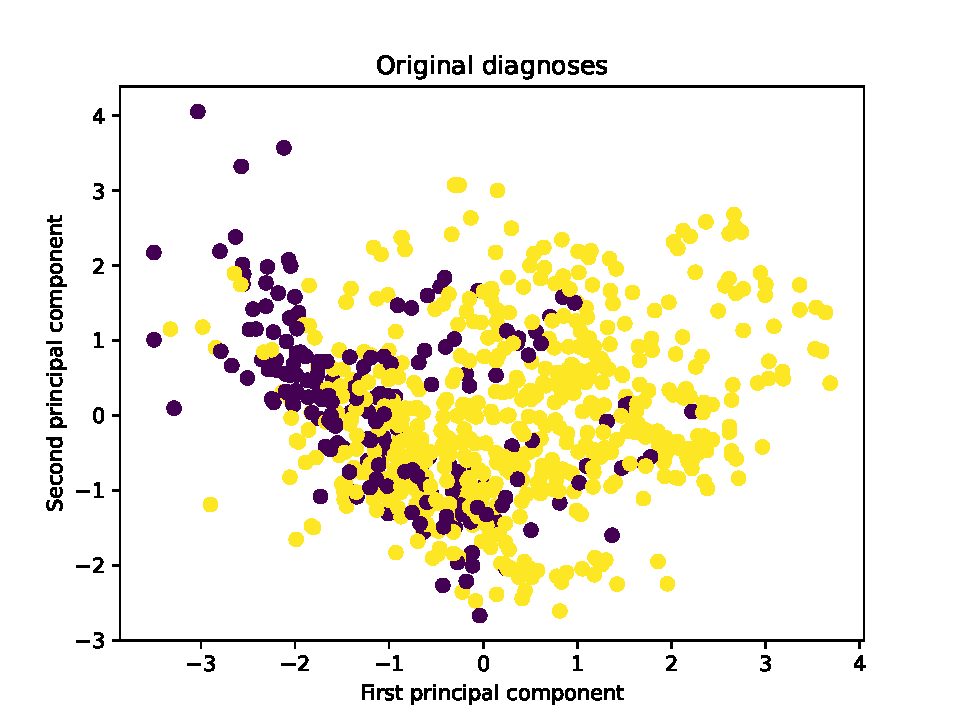
\includegraphics[scale=0.6]{hw04_plot_pca_km1.pdf}
     &
    \vspace{-4mm}\hspace{-5.25mm}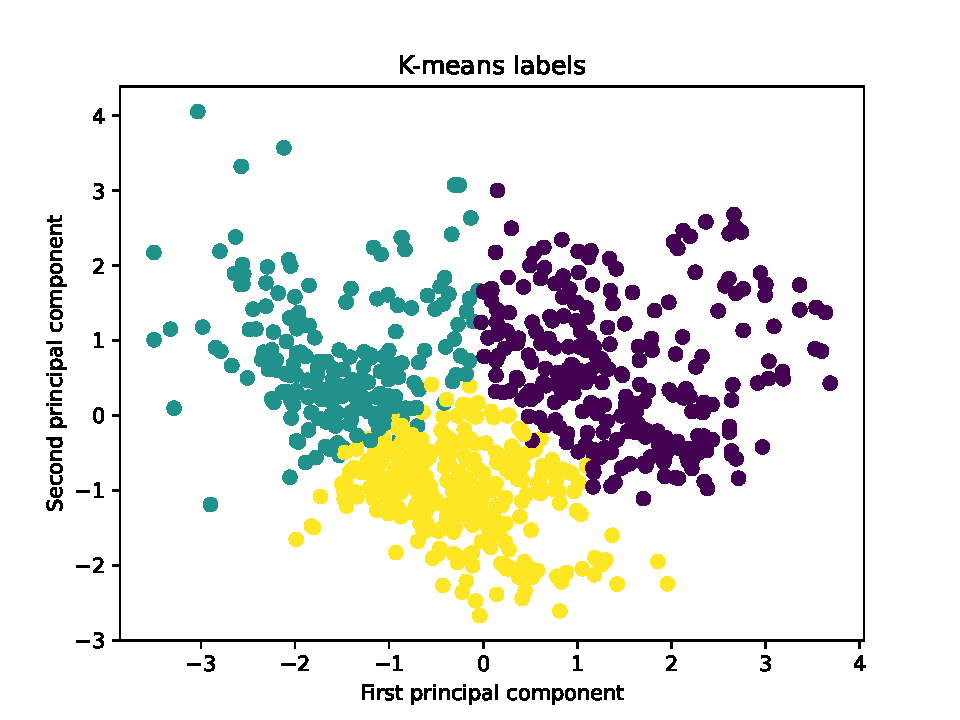
\includegraphics[scale=0.6]{hw04_plot_pca_km2.pdf}
  \end{tabularx}
\end{flushleft}

% PROBLEM 4
\begin{flushleft}
  \textbf{4)} The number of components needed to account for 80\% of the variance is 31. We can conclude that the first principal component explains almost 100\% of the variability, and thus it is sufficient to explain the requested 80\%. \par
  \vspace{-1mm}
  \begin{center}
    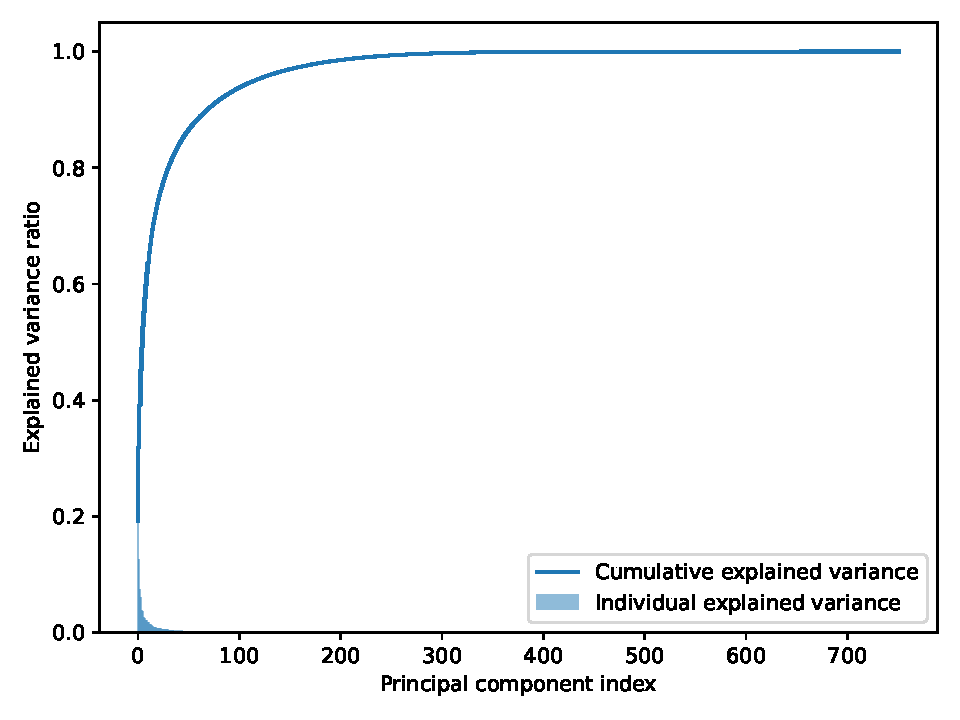
\includegraphics[scale=0.6]{hw04_plot_pca_variance.pdf}
  \end{center}
\end{flushleft}

\pagebreak
\hspace{-8.25mm}
\color{darkgray}
\renewcommand\tabularxcolumn[1]{m{#1}}
\begin{tabularx}{1.09\textwidth} {>{\raggedright\arraybackslash}X >{\centering\arraybackslash}X >{\raggedleft\arraybackslash}X}
  
\includegraphics[scale=0.2]{tecnico.pdf}                           &
  \textbf{Aprendizagem 2022/23} \par \textbf{Homework IV - Group 66} &
  João Cardoso, 99251 \par José João Ferreira, 99259
\end{tabularx}
\renewcommand\tabularxcolumn[1]{p{#1}}
\color{black}

\begin{center}
  \textbf{III. Appendix}
\end{center}

\definecolor{backcolour}{rgb}{0.95,0.95,0.92}
\definecolor{codegreen}{rgb}{0,0.6,0}
\definecolor{codepurple}{rgb}{0.58,0,0.82}
\definecolor{codegray}{rgb}{0.5,0.5,0.5}
\definecolor{codered}{rgb}{0.75,0.25,0}
\definecolor{codeyellow}{rgb}{0.55,0.55,0.0}
\definecolor{codeForestGreen}{rgb}{0.05,0.65,0.55}

\lstdefinestyle{mystyle}{
  backgroundcolor=\color{backcolour},
  commentstyle=\color{codegreen},
  keywordstyle=\color{codepurple},
  numberstyle=\tiny\color{codegray},
  stringstyle=\color{codered},
  emph=[0]{loadarff,silhouette_score,drop,fit_transform,array,fit_transform,fit,silhouette_score,contingency_matrix,max,print},
  emphstyle=[0]\color{codeyellow},
  emph=[1]{pandas,pd,numpy,np,scipy,io,arff,sklearn,preprocessing,LabelEncoder,MinMaxScaler,metrics,cluster,KMeans,metrics,DataFrame,range,PCA,decomposition,matplotlib,pyplot,plt},
  emphstyle=[1]\color{codeForestGreen},
  basicstyle=\ttfamily\footnotesize,
  breakatwhitespace=false,
  breaklines=true,
  captionpos=b,
  keepspaces=true,
  numbers=left,
  numbersep=7.5pt,
  showspaces=false,
  showstringspaces=false,
  showtabs=false,
  tabsize=2,
  language=Python,
  morekeywords={as}}
\lstset{style=mystyle}

\hspace{-8.25mm}
\begin{tabularx}{1.09\textwidth}{X}
  \lstinputlisting{hw04_1.py}
\end{tabularx}

\pagebreak
\hspace{-8.25mm}
\color{darkgray}
\renewcommand\tabularxcolumn[1]{m{#1}}
\begin{tabularx}{1.09\textwidth} {>{\raggedright\arraybackslash}X >{\centering\arraybackslash}X >{\raggedleft\arraybackslash}X}
  
\includegraphics[scale=0.2]{tecnico.pdf}                           &
  \textbf{Aprendizagem 2022/23} \par \textbf{Homework IV - Group 66} &
  João Cardoso, 99251 \par José João Ferreira, 99259
\end{tabularx}
\renewcommand\tabularxcolumn[1]{p{#1}}
\color{black}

\begin{center}
  \textbf{}
\end{center}

\hspace{-8.25mm}
\begin{tabularx}{1.09\textwidth}{X}
  \lstinputlisting{hw04_3.py}
\end{tabularx}

\hspace{-8.25mm}
\begin{tabularx}{1.09\textwidth}{X}
  \lstinputlisting{hw04_4.py}
\end{tabularx}

\end{document}